\documentclass[10pt]{beamer}

\usetheme[progressbar=frametitle]{metropolis}
\usepackage{appendixnumberbeamer}

\usepackage{booktabs}
\usepackage[scale=2]{ccicons}

\usepackage{pgfplots}
\usepgfplotslibrary{dateplot}

\usepackage{xspace}
\newcommand{\themename}{\textbf{\textsc{metropolis}}\xspace}

\setcounter{tocdepth}{1}

\title{Cheating complexity}
\subtitle{Electronic structure the easy way}
% \date{\today}
\date{}
\author{Jacob Ross}
\institute{RSPE invades RSC}
% \titlegraphic{\hfill\includegraphics[height=1.5cm]{logo.pdf}}

\begin{document}

\maketitle

\begin{frame}{The journey ahead}
  %\setbeamertemplate{section in toc}
  \tableofcontents
\end{frame}

\begin{frame}{But first...} 
Some disclaimers:
\begin{itemize}
    \item I'm not a theorist, just an enthusiastic amateur.
    \item This is an exposition, not original research.
    \item Participation is welcome.
\end{itemize}%This could be considered an exposition
%On a collection of results that are not mine. There's no new research, just a collection of ideas that I think are pretty beautiful. I'm grateful for the opportunity.
%Most of what I'll say pertaining to electronics is in reference to strongly correlated systems. Quantum chemistry is a ways outside my expertise - but many of the ideas will translate, I hope.
    
\end{frame}


\section{Everything you need to know about Hamiltonian mechanics}
\begin{frame}{Physics: The classical picture}
The basic \emph{ontology} of classical Hamiltonian physics consists of:
    \begin{itemize}
        \item A \emph{system} whose \emph{state} specified by a set of N canonical coordinates $q_i$ and N canonical momenta $p_i, i\in\{1,\dots,N\}$. %These live in the tangent space of a manifold
        \item The \emph{equations of motion} whose solutions, given initial or boundary data, specify the trajectory of the system over time. 
    \end{itemize}    
The equations of motion can be obtained from Hamilton's equations, 

$$ \dot{q_i} = \frac{\partial H}{\partial p_i}, \dot{p_i} = -\frac{\partial H}{\partial q_i} $$

Where $H(\textbf{q},\textbf{p})$ is the \emph{Hamiltonian}, a distinguished function on the configuration space of the system.  %which is to say, on the Tangent bundle of a smooth manifold with a Symplectic form; contrast with the path-integral or Lagrangian approach which requires boundary value data. Still, Hamilton's formulation is equivalent to the stationary-action Lagrangian approach.
\end{frame}

\begin{frame}{Physics: The classical picture}
The \emph{epistemology} of classical physics assumes:
\begin{itemize}
    \item All observables are \emph{functions} on the configuration space %$O(\textbf{q},\textbf{p})$, eg kinetic energy $K= \frac{\textbf{p}^2}{2}$, angular momentum $L = \textbf{q}\times \textbf{p}$. 
    \item Observables (including coordinates) evolve following differential equations obtained through the Poisson bracket,
    
    $$ \{O,H\} = \frac{d O}{d t}  = \frac{\partial O}{\partial \textbf{q}}\frac{\partial H}{\partial \textbf{p}}-\frac{\partial H}{\partial \textbf{p}}\frac{\partial O}{\partial \textbf{q}}$$
    
    \item \emph{Measurement} of the system is a direct reading-out of the value of an observable $O$ at the point $p,q$ specifying the current state of the system
    
    \item \emph{Probability distributions} are $L^1$ positive-semidefinite functions on the configuration space whose volume is preserved during time evolution.
\end{itemize}

\end{frame}
%I run over the classical picture to emphasize the similarity in spirit, if difference in structure, between the Hamiltonian formulation of classical mechanics and the modern Matrix formulation of quantum physics. 

\begin{frame}{Many-body Physics: The Classical Picture}

For a collection of $i$ systems each of dimension $d_i$, the state is completely specified by an element in the \emph{Cartesian product} of the constituent configuration spaces, 
$$T = T_A\times T_B =\{a\in A, b\in{B}\}$$
which has dimension $D = \sum_i d_i$. %Refer to Feynman's notes. Have I got this all wrong? 
\end{frame}

\begin{frame}{The quantum picture}
All of the physical information in the system is encoded by the wavefunction $|\psi\rangle$.

$$|\psi\rangle \in H = \mathbb{C}^d$$ 
% H complete vector space with norm \& inner product of integer dimension $d$. 

    Observables correspond to \emph{linear operators} on the Hilbert space $H$. 
    
    \emph{Hermitian} operators, $A^\dagger = A$, have a \emph{complete orthonormal basis} of so-called eigenstates $|a_i\rangle$. These correspond to different measurement outcomes, and their observed values correspond to the eigenvalues of the corresponding operator.
    
    The probability of a given outcome $a_i$ is given by $|\langle a_i|\psi\rangle|^2$.
    In the basis of eigenvectors of $\hat{A}, A = \sum_i \alpha_i |a_i\rangle\langle a_i| = \textrm{diag}(\alpha_i)$.
    
    The expectation value of an outcome is given by $\langle O \rangle = \sum_s p_s O_s = \langle\psi|\hat{O}|\psi\rangle$

\end{frame}
\begin{frame}{The quantum picture}

The time evolution is governed by the (time-dependent) Schr\"{o}dinger equation,
$$  i \hbar\frac{\partial |\psi\rangle}{\partial t} = \hat{H} |\psi\rangle$$
With solution
$$ |\psi(t)\rangle = U(t)|\psi(0)\rangle$$
The Hamiltonian $\hat{H}$ is a self-adjoint linear operator on $H$
    
    The expectation value of an observable evolves by the Commutator $d O/d t = \frac{i}{\hbar}[H,O]$ if the Hamiltonian is time-independent.
    
\end{frame}

\begin{frame}{The quantum picture}
    In the basis of eigenvectors of H,

\begin{align*}
    H|\psi(t)\rangle &= i\hbar \partial_t|\psi(t)\rangle\\
    &= H\sum_i c_i|e_n\rangle\\
    &= \sum_i c_i E_n |e_n\rangle\\
\end{align*}
Which gives a matrix equation with solution $|\psi(t) \rangle = e^{iHt/\hbar} |\psi(0)\rangle = \sum_n e^{i E_n t/\hbar} c_n |e_n\rangle$

%hence the name stationary states, and the definition of the TDSE singles out the Hamiltonian from the set of possible operators.
\end{frame}

\begin{frame}{Many-body physics}
The Hilbert space of a composite system consisting of subsystems $A$ and $B$ is the \emph{tensor product}.
$$ H_{AB} = H_A\otimes H_B$$
which has dimension $D = d_a \times d_b$!

It contains
\begin{itemize}
    \item Separable states $$ |\Psi_{AB} \rangle =  |\psi_{A}\rangle \otimes |\psi_{B}\rangle. $$
    \item Non-separable (\emph{entangled}) states.
\end{itemize}

%It also has a remarkable structure. In addition to containing, apparently, more information than a classical composite system (but too bad, n qubits can only ever give you n bits), it also includes states which can be written as something like a Cartesian product
%Why the tensor product?

\end{frame}

%And there you have it, chemistry solved. Wait, no. You must expend computational effort (and real effort) to make predictions using these compressions of the patterns observed in nature. Sometimes we're lucky, like in the Hydrogen atom or the harmonic oscillator or the periodic potential, but in very many cases there's nothing better than a wall of GPU.

\begin{frame}{Why computation is useful}
\begin{itemize}
    \item ``Laws of nature" are artefacts of a great deal of compression
    \item To predict the future, we must expend computational effort
    \item Closed-form solutions are rare
    \item Therefore, we confront the problem of simulation
    %\item Simulation is the controllable representation of a system with meaningful, relevant output
\end{itemize}
\end{frame}
%%%%%%%%%%%%%%%%%%%%%%%%%%%%%%%%%%%%%%%%%%%%%%%%%%%%%%%%%%%%%%%%%%%%%%%
\section{Why is quantum physics hard?}
\begin{frame}{Why is quantum physics hard?}

Performing a simulation requires, roughly,
\begin{itemize}
    \item State representation
    \item State preparation (input)
    \item Time evolution 
    \item State observation (output)
\end{itemize}

In three categories:
\begin{itemize}
    \item Classical digital computing
    \item Digital quantum computing
    \item Analog quantum simulation
\end{itemize}

%We'll try to see three methods to deal with this: Classical digital computing, quantum digital simulation, and analog quantum simulation.
    
\end{frame}

\begin{frame}{Why is quantum physics hard?}
For each parameter $s_n$ (coefficients or canonical coordinates), take binary approximations

$$\sigma_n = \sum_{k=1}^N 2^k\times a_n \approx  \sum_{k=1}^\infty 2^k\times a_n= s_n,$$ 

Encoding a composite classical system needs $2^N*n*d$ bits

Encoding a composite quantum system needs $2^N\times d^n$ bits!

%This is our first so-called obstruction to simulation. The exponential scaling of the many-body wavefunction is the reason we need algorithms like the Hartree-Fock family, which approximate the many-body wavefunction with a \emph{truncated} wavefunction in a truncated hilbert space
\end{frame}



%%%%%%%% Detour to the sign problem
\begin{frame}{Monte Carlo}

Computing high-dimensional integrals is exponentially complex.

%So what I talked about above is all well and good if you want to solve for a single trajectory. But what if you want to run an ensemble average over such things in dimensions this large? The sums you'd need to take (to approximate phase space integrals?) quickly become intractable. A 'standard workhorse' of numerical methods: Monte Carlo techniques. 

Monte Carlo methods attempt to mitigate this.

%The Monte Carlo approach is based on what's called the Metropolis algorithm, which, ideally, approximately samples from some probability distribution. The canonical application is to perform a random walk in the unit square inscribed with a circle to compute pi. It works because the random walk is \emph{ergodic} as the number of samples increases: It uniformly samples the available space. This is much more efficient than discretizing and sampling, which requires too many resources (exponentially many? For P pixels in each dof, you have $P*n^N$ bits?). You can show that the estimated value of the integral converges to the actual value with statistical error that shrinks polynomially with the number of samples. 

Provably polynomial scaling in both numerical error and time cost!

$$f(x) \approx \bar{f}(x) = \frac{1}{N}\sum_i f(x_i)$$
Gaussian distributed (by central limit theorem!) with variance $\sigma^2/N$ and statistical error scaling with $1/\sqrt{N}$. 
%Example: Computing pi with a shotgun

%So you trade accuracy for efficiency, and in practise you can shrink your numerical error below a lot of experimental error budgets: Except in some very specific and very interestingcircumstances. 
\footnote{\emph{Quantum Monte Carlo approaches for correlated systems}, Becca \& Sorella}

\end{frame}



\begin{frame}{Monte Carlo: Classical}
%The sign problem arises in the context of Monte Carlo approaches to quantum physical problems.
In classical statistical approaches, we sample from a Boltzmann-like probability distribution

\begin{align*}
    \langle O\rangle &= \sum_i O(x_i) \frac{\exp(-\beta \epsilon_i)}{\Omega},\\
    \Omega &= \sum_i \exp(-\beta \epsilon_i)
\end{align*} 

For large systems, direct sampling over the states can be impossible. Instead, generate an \emph{ergodic random walk} through the configuration space. 
\footnote{\emph{Quantum Monte Carlo approaches for correlated systems}, Becca \& Sorella}

\end{frame}

\begin{frame}{Monte Carlo: Quantum}
%Where the $\epsilon$ are the effective energies of a state (Free energy?) and $Z$ is the partition function. If you have the partition function your job is done. But if you don't, then you can generate samples from this distribution by the Metropolis-Hastings algorithm: Generate a new state via your Transition matrix, and then accept or reject the new state if the new state has lower or higher (subject to the Boltzmann ratio test) energy.
%So this is cool; With enough initial conditions this will tend to converge to an ergodic sample, and decreasing the effective temperature causes the walker to localize and sample the minima more thoroughly. 
In \emph{quantum} monte carlo, we compute expectation values of low-lying energy states by:

\begin{align*}
    \langle O \rangle& =  \frac{Tr(O \exp(-\beta H))}{Tr(\exp(-\beta H))} \\
\end{align*}  

Monte carlo approaches can work, but require mapping to a classical partition function.

Unfortunately, this is sometimes subject to the \emph{sign problem}

%Obviously this is a very different beast to the classical case, from the structural perspective, but translating this into a classical distribution is required for a monte carlo simulation. This seems to be a piece of folklore - people state it but I've not found a good exposition. The point being that in certain cases, in translating back to the classical from, you find some $x_i$ will have $P(x_i) < 0$, or even $P(x_i) \in \mathbb{C}$! 

%It's not clear in what conditions you have a sign problem. Open question! But there have been some 

%The upshot here is that statistical errors now grow without bound as the number of samples increases.

%So when is this a problem?


\end{frame}


\begin{frame}{The sign problem}
What is a sign problem?

\begin{center}
    Negative Boltzmann weights lead to unbounded errors.
\end{center}
%Indeed, there is always some operation to diagonalize the hamiltonian and produce a classical partition function. However, it requires nonlocal operations and exponential resources, which defeats the purpose

The sign problem has been demonstrated for both fermionic and bosonic systems. 

The sign problem is provably unavoidable in some cases, with intriguing connections to gravitation, and a topological origin.\footnote{\emph{Quantized gravitational responses, the sign problem, and quantum complexity}, Ringel \& Kovrizhin, Science Advances 3, (2017)}

When does a system have a sign problem? 

\begin{center}
Open question!
\end{center}

%The short answer is, we don't know exactly. There's a lot of literature that I've not had time to read and less that I have but still don't understand, but the upshot is that this is still active reserach. So Originally, the sign problem was encountered in fermionic problems, but has since been identified in bosonic ones, albeit those with a particular interaction with gravity. For exposition I'll just comment on the fermionic case because it's the most relevant and it's relatively intuitive. In computing expectation values, you solve various (imaginary time) trajectories from a stochastic sampling of your initial configurations, as in monte carlo. But if along the way you permute two of the fermions, your wavefunction picks up a negative sign (that's the exclusion principle) and therefore your computed boltzmann weight comes out negative. The reality is that the problem is much more subtle than this: If you look at the formulae carefully, you'll notice that in the Energy eigenstate basis there's no problem. But this presupposes a solution to the exponentially hard problem you're trying to solve! Moreover, it was shown that a generic solution to the sign problem is, in fact, NP-hard. This is actually quite important, and so I'll spend a moment on it.

%If there's one thing you take from this talk, maybe it should be this: The reason your subject matter is hard to compute seems to be intimately connected to some very deep ideas at the intersection of physics \& computability, which governs the domain of the possibly realizable processes within nature. Deep stuff, and the most exciting part about researching for this talk has been realizing how little we understand about this problem. 

\end{frame}

%%%%%%%% Detour to the sign problem

%The sign problem
%%Fermionic, bosonic
%%gravitational & topological origins



\begin{frame}{Quantifying complexity}
    The computational complexity of an algorithm is a measure of the computational resources requires to complete a given task.
    
    %The underlying ontology is left as an exercise to the reader
   % In the above, require an amount of memory that scales exponentially with the number of particles in the classical case. 
    %We can also talk about time-complexity, loosely the number of operations required to perform a computation, or the minimum depth of a circuit?
    %For example: Brute-force matrix multiplication scales as the cube of the input matrix size. Factoring prime numbers is not actually exponentially explosive, but it's not been proven sub-polynomial. 
    There are other kinds of tasks beyond arithmetic we might as a computer to do.

Complexity classes are defined in terms of \emph{asymptotic} resource requirements.

There are about as many classes as there are elements (don't quote me on that).
    %The upshot is that if we want to talk about efficient simulation, a reasonable heuristic is Feynman's, "If doubling the
%volume of space and time means I'll need an exponentially larger computer,
%I consider that against the rules (I make up the rules, I'm allowed to do
%that). " which we'll formalize a little bit later.
\end{frame}

%'`I know, I know: We have all these complexity classes, and they seem kind of esoteric. Maybe it's just a bad historical accident that we use all of these acronyms to express our ideas, rather than coming up with sexy names like `black hole', `quark', or `supersymmetry' as a physicist would. It's like the joke about the prisoners where one of them calls out `37' and all of them will fall on the floor laughing, then another calls out `22' but no one will laugh because it's all in the telling. There are these staggering, mind-bending mysteries about truth, proof, computers, physics, and the very limits of the knowable, and for ease of reference we bottle the mysteries up using inscrutable sequences of three or four capital letters. Maybe we shouldn't do that"
\begin{frame}{Quantifying complexity} %reword if we have to compress the sign problem
%It would be foolish to attempt to count all the complexity classes. There are just about as many identified as there are elements in the periodic table! But what is a complexity class? Well, it hinges on the idea of asymptotic complexity that we covered earlier. The most intuitive way to understand them is: For how does the computational cost required for an algorithm to terminate scale with the size of the input? Here a resource could be time, or it could be something else like memory, entanglement, or heat output. But for our purposes we'll be concerned with the time-complexity. The most obvious example is P, or polynomial-time algorithms.



Some important complexity classes: P, NP, BPP, BQP, \#P. %inclusion relations?

%Examples: Matrix multiplication, prime factoring
%Note that P here is slightly different to our polynomial-scaling functions. This actually refers to a decision problem for a turing machine, which is a very different creature but the details aren't really the point.


%The other most famous complexity class is NP. This stands for the cryptic "nondeterministic polynomial". This refers to a hypothetical branching architecture where your computer gets to employ a new processor at every conditional statement and execute all branches simultaneously. If your algorithm terminates with depth polynomial in N, AND a deterministic machine can verify whether a solution is correct in polynomial time, then you're in class NP. 

%It seems pretty intuitive that this is more complex than P. But that's not known. Indeed, there's a million dollar bounty from the Clay Mathematics institute for the answer to this question. 

An algorithm A is said to be complete for a complexity class C if every other algorithm in the class C can be reduced to A.

Wait... Why does this matter?
\begin{center}
    A generic solution to the sign problem would imply P = NP.\footnote{\emph{Computational complexity and fundamental limitations to fermionic quantum Monte Carlo simulations}, Troyer \& Wiese, PRL 94 (2005)}
\end{center}

%Finally, An algorithm A is said to be C-complete if every other algorithm in the class C can be reduced to A with at most a resource cost which is polynomial in the input size. So an NP-complete problem could be seen as a kind of 'hardest' problem in NP, which allows you to solve any NP problem using this algorithm and some polynomial overhead. Finding a generic solution to the sign problem is NP complete. That is, if you find a general solution to the sign problem that is computationally efficient, you've just shown that P = NP. 


\end{frame}


\begin{frame}{Why does this matter?}
    ``Look, this P versus NP problem, what can I say? People like to describe it as `probably the central unsolved problem in computer science.' That's a comical understatement. P vs NP is one of the deepest questions human beings have ever asked... If NP problems were  feasible, then mathematical creativity could be automated. The ability to check a proof would entail the ability to find one. Every Apple II, every Commodore, would have the reasoning power of Archimedes or Gauss. So by just programming your computer and letting it run, presumably you could solve not only P vs NP, but \emph{also the other six Clay problems.}'' -- Aaronson
\end{frame}

%\begin{frame}{Possible detour: Boson Sampling}
%    \begin{itemize}
%        \item If we have time and it fits the narrative
%        \item \#P-completeness?
%    \end{itemize}
%\end{frame}



\section{Quantum simulation in near-term technologies}

%So, the short answer to 'why is simulating quantum systems hard?' seems to be 'we don't know'. But, to be pithy, nature doesn't seem to need to pause for an exponential time between scattering events! Or, maybe it does, but that's just not visible to us inside the simulation. Digressions aside, some very clever people identified the apparent complexity in quantum physical problems and realized we can turn it to our advantage. Indeed, more recently, there is an active research program to try and identify and characterize the nature of the resources for computing that are made available by the structure of quantum physics. The rest of this talk is basically dedicated to the realization of quantum computers, in grossly sweeping terms, and emphasis on two points: One, the nature of the problem of quantum simulation, and two, the kinds of problems we might expect to be able to solve in near-term quantum devices. 




\begin{frame}{A brief history}

``Can physics be simulated by a universal computer?" - Feynman, 1982\footnote{Simulating physics with computers, IJTP 21, 1982}


``Yes." - Lloyd, 1996\footnote{Universal Quantum Simulators, Science 273, 1996}
 %Central advantage is locality - as anything consistent with SR/GR is - which means that arbirary physical (local) unitaries can be implemented efficiently 


``Will quantum computer for \$\$\$" - Everyone, 2017

\end{frame}

\begin{frame}{Quantum simulation}

There are two major paradigms for quantum computing:

\begin{itemize}
    \item \emph{Digital} quantum computing is shooting for universality, and making ground in simulation along the way.
    \item \emph{Analogue} quantum simulators have achieved great progress in specific circumstances.
\end{itemize}

%    \item State representation?
%    \item State preparation (input)?
%    \item Time evolution ?
%    \item State observation (output)?

\end{frame}
%I'll start with Analog

\begin{frame}{Analogue platforms}
    \begin{itemize}
        \item Optical Lattices \footnote{Quantum simulations with ultracold atoms in optical lattices, Gross \& Bloch, Science 357 (2017)}
        \item Trapped ions \footnote{Quantum simulations with trapped ions, Roos \& Blatt, Nat Phys 8, 2012}
        \item Superconducting qubits \footnote{On-chip quantum simulation with superconducting circuits, Houck et al, Nat Phys 8, 2012}
        \item Optical computing 
    \end{itemize}
\end{frame}

\begin{frame}{Optical Lattices}
    %Following Jaksch and Zoller's seminal proposal, Greiner \& Bloch demonstrated an \emph{optical lattice simulator} %This is the closest to my PhD. The extremely short version is you use laser cooling to produce a gas of ground-state atoms then load them into a periodic potential synthesized by a laser standing wave. 
    
    \includegraphics[width=\textwidth]{lattice_pic.jpg}
    

    %State preparation: Laser cooling & adiabatic loading

    %Observation: First, interfernce pattern (a la crystal diffraction). Nowadays, single-site and spin readout!
    
    %My PhD: Single-atom momentum resolution
\end{frame}

\begin{frame}{Optical Lattices}
 
\includegraphics[width=\textwidth]{MI_pic.png}
    %State representation: Depends what you're simulating. For a magnetic problem, use the sitewise spin of a unity-filled lattice. For a conduction problem, you're concerned with transport properties of the atoms through the lattice.
    %Time evolution: Built-in to light potential - hamiltonian engineering!
    
%Modern achievements: Lattice microscopes, Disordered lattices, Heisenberg Antiferromagnet,Gauge theories, Thermalization, topological physics...
%Around the corner: Quasicrystals, long-range interactions, quantum gates? Hall effect? Superconductivity?

\end{frame}


\begin{frame}{Simulations for Quantum chemistry}
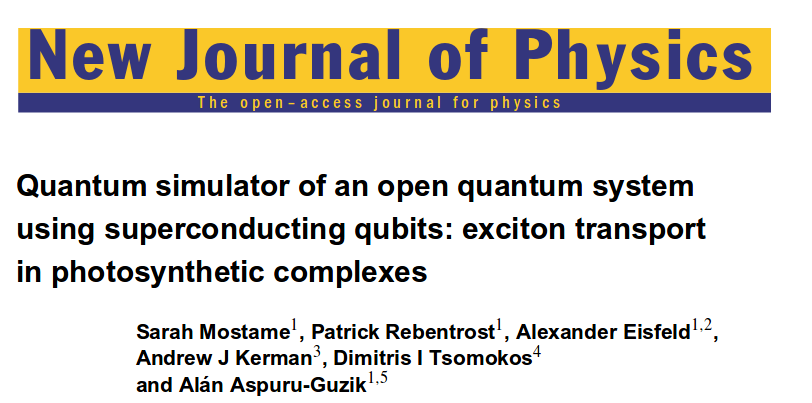
\includegraphics[width=\textwidth]{photosynthesis.png}
\end{frame}

\begin{frame}{Simulations for Quantum chemistry}
    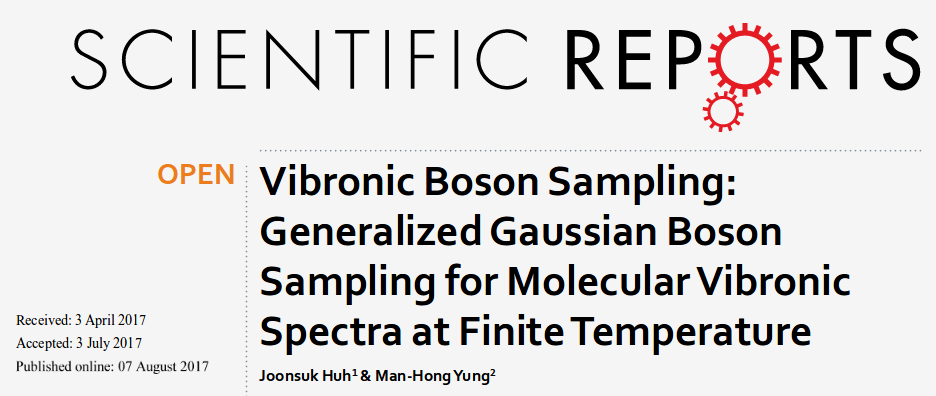
\includegraphics[width=\textwidth]{vibronic_boson_sampling.png}
\end{frame}

\begin{frame}{Simulations for Quantum chemistry}
     \includegraphics[width=\textwidth]{efficient.png}
\end{frame}



\begin{frame}{Accessible quantum computing}
Want to get your hands dirty?
    \begin{itemize}
        \item Microsoft Q\# 
        \item IQM Station Q
        \item Google OpenFermion
        \item Xanadu StrawberryFields
    \end{itemize}
\end{frame}


\begin{frame}{Perspective}%conclusion
    ``Quantum phenomena do not occur in a Hilbert space, they occur in a laboratory." - Asher Peres
    
   ``Maybe it's just a bad historical accident that we use all of these acronyms to express our ideas, rather than coming up with sexy names like `black hole', `quark', or `supersymmetry' as a physicist would. It's like the joke about the prisoners where one of them calls out `37' and all of them will fall on the floor laughing, then another calls out `22' but no one will laugh because it's all in the telling. There are these staggering, mind-bending mysteries about truth, proof, computers, physics, and the very limits of the knowable, and for ease of reference we bottle the mysteries up using inscrutable sequences of three or four capital letters. Maybe we shouldn't do that" - Scott Aaronson
    
    Quantum chemistry is about to get really interesting.
\end{frame}

\begin{frame}{}
    \begin{center}
        Thanks for having me!
    \end{center}
\end{frame}

\section{}

%\begin{frame}{Example: Observables}

%Pick a simpler example; one that exhibits entanglement though?


%system
%Observables

%Two non-interacting electrons in a harmonic oscillator have observables $\hat{S}, \hat{H},$ and each have so bases $|E, S\rangle$. Consider the singlet state (with some %abuse of notation)
%$$|\Psi\rangle  = \frac{1}{\sqrt{2}}(|0,0,\uparrow\downarrow\rangle+|1,1,\uparrow\downarrow\rangle$$
%Probabilties of outcomes: 
%\begin{align*}
 %   P(E_A = 0) &= \frac{1}{2},\\
%    P(S_B = \uparrow) &= \frac{1}{2},\\
 %   P(E_A = 0 | S_B = \uparrow) &= 0\\
%\end{align*}

%\end{frame}

%\begin{frame}{Example: Expectation values}
%Two non-interacting electrons in a harmonic oscillator have observables $\hat{S}, \hat{H},$ and each have so bases $|E, S\rangle$. Consider the singlet state (with some abuse of notation)

%$$|\Psi\rangle  = \frac{1}{\sqrt{2}}(|0,0,\uparrow\downarrow\rangle+|1,1,\uparrow\downarrow\rangle$$
%Expectation values:
%\begin{align*}
  %  \langle E\rangle &= \langle\Psi|\hat{H}|\Psi\rangle\\
%    &= \frac{1}{2}(\langle 0,\uparrow\downarrow|\hat{H}| 0,\uparrow\downarrow\rangle + \langle 1, \downarrow\uparrow|\hat{H}|1,\downarrow\uparrow\rangle)\\
 %   &= \frac{1}{2}(\hbar\omega + 3\hbar\omega)\\
 %   &= 2\hbar\omega
%\end{align*}
%\end{frame}

%\begin{frame}{Example: Time evolution}

%Two non-interacting electrons in a harmonic oscillator have observables $\hat{S}, \hat{H},$ and each have so bases $|E, S\rangle$. Consider the singlet state (with some abuse of notation)

%$$|\Psi\rangle  = \frac{1}{\sqrt{2}}(|0,0,\uparrow\downarrow\rangle+|1,1,\uparrow\downarrow\rangle$$

%\begin{align*}
   % |\dot{\Psi}\rangle &= -\frac{i}{\hbar} \hat{H}|\Psi\rangle\\
 %   &= -\frac{i}{\sqrt{2\hbar}}(\hbar\omega|0,0,\uparrow\downarrow\rangle+3\hbar\omega|1,1,\uparrow\downarrow\rangle\\
%\implies |\Psi(t)\rangle &= \frac{1}{\sqrt{2}}  (e^{-i\omega t}|0,0,\uparrow\downarrow\rangle+e^{-3i\omega t}|1,1,\uparrow\downarrow\rangle)   
%\end{align*}


%\end{frame}

%\begin{frame}{Example: Entanglement}
%Two non-interacting electrons in a harmonic oscillator have observables $\hat{S}, \hat{H},$ and each have so bases $|E, S\rangle$. Consider the singlet state (with some abuse of notation)

%$$|\Psi\rangle  = \frac{1}{\sqrt{2}}(|0,0,\uparrow\downarrow\rangle+|1,1,\uparrow\downarrow\rangle$$

%Consider sequential measurements of the spin of each particle. Then

%Which is actually a maximally entangled state! 

%Existence of some such states shows that local realism is not a correct description of reality. Entanglement is an important resource for quantum computing, information processing, and communication. 
%\end{frame}

\end{document}

